%\begin{chapterabstract}
This section describes the fundamental principles behind the Vector Packet Processing (VPP) technology, which aims to enable efficient and high-performance network packet processing. 
VPP is built on modern programming and architectural principles that allow maximum utilization of contemporary hardware, particularly in parallel processing and memory access optimization.
%\end{chapterabstract}

The section begins with a brief description of traditional network traffic processing methods used by operating systems and their limitations in terms of performance and scalability. 
Following that, the architecture of VPP is explored in detail, explaining how packets are processed in vectors, the use of a node graph, 
and the various techniques that contribute to its high efficiency -- such as I/O and compute batching, zero-copy methods, and lock-free multi-threading. 
The purpose of this section is to provide a theoretical foundation for understanding how VPP operates.

%-----------------------------------------------------
\subsection{Traditional network traffic processing}
A \textit{network packet} is a basic unit of data transmitted over a network. It consists of a \textit{header}, which includes control information such as source and destination IP addresses, 
and a \textit{payload}, which carries the actual user data. 
Packets are routed independently through the network and reassembled at the destination. 
This structure allows efficient and reliable communication, even over complex or unreliable network paths.

Currently, packet processing works as follows: a packet arrives at the network card, which then
issues a system call (syscall) to the operating system for packet processing. The microprocessor
must save the currently executing instruction, perform a context switch, locate the appropriate
service routine in the interrupt vector table, and handle the packet processing. Once completed, it
must restore the saved instruction, perform another context switch, and return to processing the
interrupted program.

This system for operating peripherals was designed under the assumption that the peripherals
would not request interrupts continuously, which is not the case with network devices that need
to process large volumes of data split into small parts. 
This method requires the microprocessor to execute a significant
number of instructions not directly related to packet processing. 
Gallatin et al.~\cite{gallatin1999trapeze} discovered 
%\footnote{kap. 3.3 obr. 6} 
that if MTU is 1500 bytes, then interrupt handling accounts for 20\% - 25\% of receiver packet-processing overhead.
Another disadvantage of tradidtional packet processing is the inefficient handling of cache memory; the processing of the packets one by one in response to
interrupts leads to frequent cache misses in both cache and inctruction caches.~\cite{cox2000profiling} 
%\footnote{kap. 4.2}

%-----------------------------------------------------
\subsection{An Introduction to VPP}

Vector Packet Processing is a multi-platform network stack that operates at layers 2-4 of the ISO/OSI model and is developed by the FD.io project. 
It consists of a set of forwarding vertices arranged in an oriented graph and auxiliary software and provides out-of-the-box switch/router functionality.
Unlike traditional network stacks, which run in the kernel, VPP operates in user space.

In a traditional approach, packets are processed one by one. In contrast, VPP reads the largest available number of packets called vector from the network interface card (NIC) 
and processes the entire vector through a VPP node-graph one node at a time. Each node in this graph handles a specific part of the packet processing.
This approach reduces cache misses and spreads fixed overhead costs across multiple packets, lowering the average processing cost per packet. 
Additionally, it allows VPP to take advantage of multiple cores, enabling parallel processing, which significantly improves overall performance.

VPP runs on common off-the-shelf hardware (COTS), ensuring its broad compatibility and flexibility for deployment. 
It supports various architectures such as x86, ARM, and Power, and can be deployed on both standard servers and embedded devices. 
The design of VPP is agnostic to hardware, kernel, and deployment platform, meaning it can operate across a wide range of systems, including bare metal servers, virtual machines (VMs), and containers. 
This approach allows VPP to be deployed on widely available infrastructure without the need for specialized hardware.~\cite{fdio_what_is_vpp}

%-----------------------------------------------------
\subsection{Techniques used in VPP}
According to Linguaglossa et al.~\cite{LINGUAGLOSSA}, 
VPP utilizes a combination of kernel-bypass and low-level code optimization techniques to maximize packet processing efficiency and take full advantage of modern CPU microarchitectures.
These techniques include:

\begin{itemize}
  \item \textbf{Lock-Free Multi-Threading}
is a programming technique that leverages modern multi-core CPUs to increase system performance. In network applications, parallelism is achieved by running multiple threads in the same time. 
Ideally, the more threads are used, the better the system performance but only up to a saturation point beyond which additional threads bring no gainns. 
However, to reach this ideal performance, traditional synchronization mechanisms such as mutexes and semaphores must be avoided, as they introduce delays due to thread contention. 
Instead, lock-free architectures have to be used, allowing threads to operate independently without blocking each other. 
In the context of VPP this approach is enabled by hardware features like multi-queue NICs, 
which allow each thread to handle a distinct subset of traffic, ensuring efficient and parallel processing.~\cite{LINGUAGLOSSA}

  \item \textbf{I/O batching}
is a key technique used in VPP. 
Instead of raising an interrupt for every incoming packet, the network interface card collects multiple packets into a buffer and triggers an interrupt only when the buffer is full. 
This reduces the overhead caused by frequent context switching and interrupt handling. 
VPP typically uses poll-mode drivers, which collect packets in batches without relying on interrupts. 
Moreover, the batching technique is applied system-wide in VPP. 
This approach maximizes CPU efficiency, improves cache usage, and delivers stable, high-throughput performance even under heavy load.~\cite{LINGUAGLOSSA}

  \item \textbf{Compute batching} 
is a technique that extends I/O batching to the processing phase itself. 
Instead of processing one packet at a time, network functions are designed to operate on entire batches of packets. 
This approach minimizes overhead from function calls (such as context switches and stack setup) and improves instruction cache efficiency. 
When a batch of packets enters a processing function, only the first packet might cause an instruction cache miss, while the rest benefit from the already warmed cache.
Additionally it is possible to take advatage of instruction-level parallelism.~\cite{LINGUAGLOSSA}
  
  \item \textbf{Receive-Side Scaling}
is a hardware-based technique used by modern NICs to distribute incoming packets across multiple RX queues. 
This enables parallel packet processing by allowing each queue to be handled by a separate thread, improving scalability and throughput. 
Packet assignment is typically done using a hash function over packet header fields (e.g., the 5-tuple).~\cite{LINGUAGLOSSA}

  \item \textbf{Zero-Copy} 
is a technique used to eliminate unnecessary memory copying during packet processing. 
Instead of copying incoming packets from the network interface card to a separate buffer via system calls, 
the NIC writes packets directly into a pre-allocated memory region that is shared with the user-space application via Direct Memory Access (DMA). 
This allows the application to access packet data without invoking system calls or duplicating memory, which greatly reduces CPU overhead.~\cite{LINGUAGLOSSA}
 
  \item \textbf{Multi-loop} is a coding technique in which functions are designed to process \textit{N} packets simultaneously, assuming they undergo the same operations. 
Because the processing of each packet is usually independent of the others, this approach enables high instruction-level parallelism and keeps CPU pipelines efficiently utilized. 
It requires writing explicitly parallel functions, often using C templates, and helps increase throughput by raising the number of instructions executed per clock cycle. 
However, its effectiveness is limited when performance is primarily constrained by memory access rather than computation.~\cite{LINGUAGLOSSA}

  \item \textbf{Data prefetching} is a technique used to preload data into the CPU cache before it is actually needed during processing. 
In the context of VPP, this means prefetching data for the \textit{i+1}-th packet while the \textit{i}-th packet is being processed.
When combined with multi-loop processing, it is possible to prefetch data for packets \textit{i+1} to \textit{i+N} while processing packets \textit{i−N} to \textit{i}, further improving efficiency.
Although prefetching cannot be applied at the start or end of the batch (due to a lack of preceding or following packets), 
this limitation has negligible impact on performance because of the large batch size (usually 256 packets) typically used in VPP.
The technique increases instructions per clock cycle by reducing memory access latency.~\cite{LINGUAGLOSSA}

 \item \textbf{Branch prediction} in VPP refers to a coding practice where developers provide compiler hints to indicate which branch of a conditional statement is more likely to be taken.
These hints allow the compiler to generate optimized machine code that minimizes the performance cost of mispredicted branches.
When the prediction is correct, the CPU pipeline continues execution without interruption, reducing wasted cycles and improving throughput.
Although modern CPUs have effective built-in branch predictors, providing explicit hints can still offer performance benefits in branch-heavy code.
Because the processing logic in VPP is relatively stable, such predictions are often accurate and help to improve performance.~\cite{LINGUAGLOSSA}
 
  \item \textbf{Function flattening} refers to the use of inline functions within VPP graph nodes to eliminate the overhead associated with standard function calls.
By avoiding register shuffling and stack operations required by the Application Binary Interface, this approach reduces latency and improves execution speed.
Additionally, inlining enables the compiler to perform more aggressive optimizations, such as removing unused code branches.~\cite{LINGUAGLOSSA}

  \item \textbf{Direct Cache Access} is a hardware-supported technique that allows network interface cards to write incoming packet data directly into the CPU’s L3 cache, bypassing RAM. 
As an extension of zero-copy using DMA, this reduces memory latency and can significantly reduce RAM usage.~\cite{LINGUAGLOSSA}

  \item \textbf{Multi-architecture support} allows VPP to select the most suitable implementation of a graph node function at runtime, based on the detected CPU microarchitecture.
For example, a single binary can dynamically use AVX2-optimized code on supported processors, while falling back to compatible versions on older hardware.~\cite{LINGUAGLOSSA}
  
  \item \textbf{Cache Coherence and Locality} are critical factors in the performance of modern software-based packet processing systems. 
In current COTS architectures, memory access has become a major bottleneck, which is mitigated by a multi-level cache hierarchy.
Minimizing cache misses and maintaining data locality during packet processing is essential for achieving high performance and low latency.~\cite{LINGUAGLOSSA}

\end{itemize}

%-----------------------------------------------------
\subsection{VPP Processing Graph and Graph nodes}
At the core of VPP lies the Packet Processing Graph, a directed graph composed of relatively small, modular and loosely coupled nodes. 
Each node is designed to perform a specific task and there are 3 types of them: \textit{process}, \textit{input} and \textit{internal}. 
Process nodes do not participate in the packet forwarding graph; instead, they handle timers, events, and other background tasks within the VPP runtime.
Input nodes are used for input of data and internal nodes are used for vector processing. Internal nodes also serve as output nodes. 
When a vector of packets is prepared by input node, it is then pushed through the internal nodes. 
During processing, the vector may be split if the batch contains packets of different protocols or types, as they may need to follow different paths through the graph.
When the original vector is completely processed, the process repeats.
Illustration of this Processing Graph is shown in fig. \ref{fig:processing-graph}.

\begin{figure}[!htbp]
    \centering
    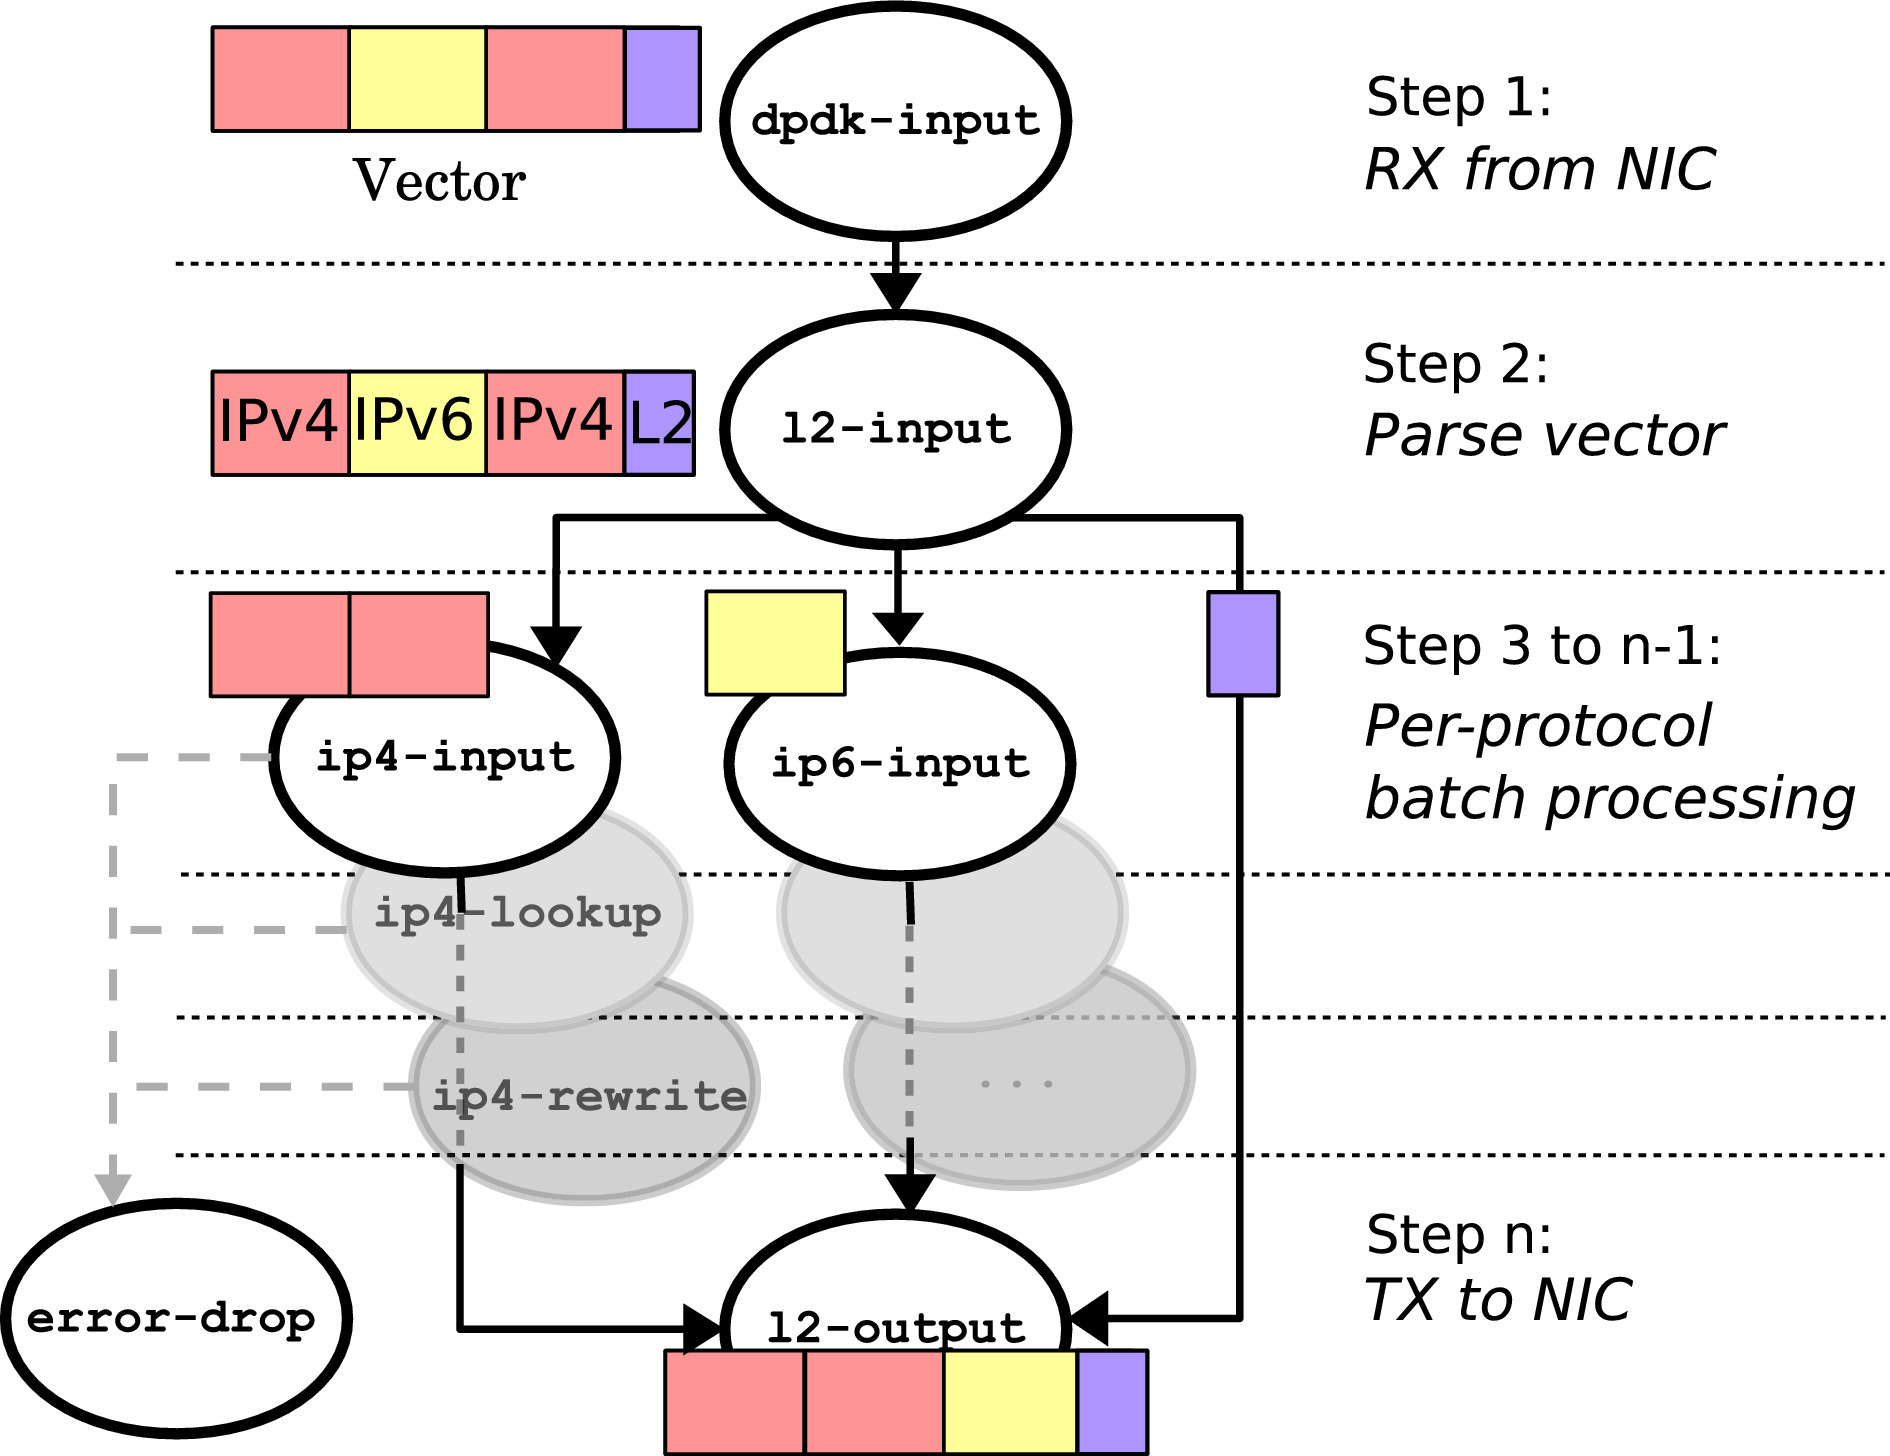
\includegraphics[width=0.85\linewidth]{images/processing-graph.jpg}
    \caption{Picture showing the VPP Processing Graph~\cite{LINGUAGLOSSA}}
    \label{fig:processing-graph}
\end{figure}

Thanks to VPP's modular design, the processing graph is highly customizable and extensible. 
New nodes -- referred to as plugins -- can be easily added to implement specific functionality or repleace existing ones. 
Plugins are shared libraries that are loaded during startup of VPP, and they are not dependent on the VPP source code, allowing them to be developed independently. 
Moreover, existing nodes can be rewired to modify the packet processing logic when necessary.~\cite{LINGUAGLOSSA, DR:COMMAG-18, fdio_vpp_extensible_2021}

%--------------------------------------------------------------------
\subsection{Multithreading and Thread Roles}
VPP can operate in either single-threaded or multi-threaded mode. In single-threaded mode -- which is the default configuration -- a single \texttt{main thread} handles all functions, 
including both packet processing and management tasks.  
In multi-threaded mode, the \texttt{main thread} is responsible for management functions (such as the debug CLI, API handling, and statistics collection), 
while one or more \texttt{worker threads} handle packet processing from input to output.  

Each worker thread polls input queues on a subset of interfaces. 
When Receive Side Scaling is enabled, multiple worker threads can process different hardware queues of the same NIC in parallel.~\cite{fdio-multithreading}

%--------------------------------------------------------------------
\subsection{DPDK and Its Role in VPP}
The Data Plane Development Kit (DPDK) is an open-source collection of libraries and drivers designed to support high-speed packet processing in user space. 
It was initially developed by Intel in 2010 and is now maintained as a Linux Foundation project. 
DPDK provides a set of APIs and components that allow applications to bypass the kernel network stack and to directly access network interface cards 
through poll-mode drivers (PMD), significantly reducing the overhead associated with traditional packet handling mechanisms.~\cite{dpdk_about}

DPDK is used in VPP for interfacing with hardware. It is implemented as a plugin called \textit{dpdk-plugin}.~\cite{LINGUAGLOSSA, DR:COMMAG-18} 

While VPP supports multiple mechanisms for accessing network devices, such as \textit{af\_packet}, to the best of the author's knowledge, DPDK is by far the most widely used option.

%--------------------------------------------------------------------
\subsubsection{Poll Mode Drivers}
Poll Mode Drivers (PMDs) are a key component of the DPDK framework. Unlike traditional network drivers, which rely on interrupts to signal packet arrival, 
PMDs continuously poll the network interface card -- specifically its RX queue -- in a busy-loop, completely avoiding traditional interrupt-based mechanisms. 
This approach allows packets to be retrieved, processed, and delivered directly to user space without kernel involvement. 
While this results in very low latency and high throughput, it also causes constant CPU utilization on the cores assigned to polling, regardless of the traffic load.~\cite{FREITAS2022148}

Not every network interface card is supported by DPDK. Each supported device requires a specific Poll Mode Driver, which must be available and compatible with the given hardware. 
An up-to-date list of supported NICs and their corresponding PMDs is maintained on the official DPDK website.~\cite{dpdk-supported-nics}

%--------------------------------------------------------------------
\subsubsection{Memory management and Hugepages}
DPDK uses a user-space memory model that eliminates the need for kernel involvement during packet processing. 
It operates on memory regions reserved as hugepages -- large memory pages, typically 2 MB or 1 GB in size, which are allocated at startup. 
These hugepages are used to store packet buffers and manage memory pools. 
DPDK defines its own memory management structures, such as mempools, which consist of preallocated fixed-size objects. 

DPDK is also explicitly NUMA-aware. Most memory allocation functions require the application to specify the target NUMA node, ensuring that memory is allocated close to the CPU core accessing it. 
This minimizes latency caused by cross-node memory access and helps optimize performance on multi-socket systems.~\cite{burakov2019memory}

%--------------------------------------------------------------------
\subsubsection{Packet Reception and Transmission: A comparison between Linux Network Stack and DPDK}
When a packet arrives at a NIC managed by the Linux Network Stack, it is first stored in the NIC’s internal buffers. 
The NIC then writes the packet via Direct Memory Access (DMA) to the section of RAM provided by the driver and updates the corresponding descriptor in the RX buffer. 
The RX buffer is implemented as a ring queue.

Once the packet has been saved, the corresponding interrupt request (IRQ) is triggered to notify the CPU that one or more packets have arrived in that queue. 
Then, the corresponding IRQ handler is executed, which acknowledges the interrupt and calls the \textit{napi\_schedule} and \textit{\_\_raise\_softirq\_irqoff} functions.

%broken xelatex
\newpage
The first function marks the associated \texttt{napi\_struct}%
\footnote{\texttt{napi\_struct} represents a NAPI context associated with a specific receive queue of a network device.}
 as ready for processing, while the second one raises a software interrupt (SoftIQR) specifically intended for processing incoming packets. 
Once the SoftIRQ is triggered, the kernel handles the actual packet processing in a deferred context. 
It goes through a list of network devices that have indicated pending work (i.e., their associated \texttt{napi\_struct} has been marked as ready to be processed).
and calls their associated poll functions to retrieve and process packets from the receive queues.

This happens on the same CPU core that handled the original interrupt. If the system is busy or the processing takes too long, the remaining work may be handled by the \textit{ksoftirqd} kernel thread. 
The packets may be aggregated into a single larger packet using Generic Receive Offload (GRO), or processed individually. 
In both cases, they are passed to the IP stack via the \textit{netif\_receive\_skb} function.

The transmission path is handled in a similar manner, using ring buffers, DMA, and deferred processing. 
However, unlike reception, packet transmission is initiated from the IP stack using the \textit{\_\_dev\_queue\_xmit} function. 
Depending on the qdisc in use, packets are either enqueued in the software queue or passed directly to the driver for transmission.
Once a packet is selected for transmission, the driver places a descriptor into the TX ring buffer and sets up DMA so that the NIC can read the packet data from memory.
After the NIC finishes transmitting the packet, it triggers a TX interrupt, which allows the driver to perform post-processing such as unmapping DMA buffers and freeing memory.~\cite{linux-packet-input}

When there is a NIC with multiple RX queues available, it is assigned to one of the queues based on the NIC's configuration%
\footnote{For network interface cards with multi-queue capabilities, the corresponding kernel driver often provides a module parameter to define how many hardware queues should be initialized and utilized.}.
The selection of the target queue is typically based on a hash function computed over network and/or transport layer headers.
Each queue has a dedicated IRQ, which can be assigned to specific CPU cores based on system settings. This mechanism is known as Receive Side Scaling (RSS).

When sending a packet from a NIC equipped with multiple TX queues, Transmit Packet Steering (XPS) is used to determine the appropriate TX queue.
The first option is that a CPU core is assigned specific TX queues. The other option is to use the TX queue corresponding to the RX queue from which the flow originated.
If multiple queues are eligible, a hash function is used to select the specific queue.~\cite{linux-rss}

In comparison, incoming packets in DPDK are delivered by the network interface card (NIC) using direct memory access (DMA),
which writes packet data into pre-allocated memory buffers specified by receive (Rx) descriptors.
These descriptors are organized in a circular ring (Rx queue), where the NIC populates entries at the head, while the VPP continuously polls the tail using functions such as                    
\textit{rte\_eth\_rx\_burst()}. This polling mechanism enables the VPP to retrieve multiple packets in a batch,
minimizing interrupt overhead and reducing latency, thereby increasing throughput and core efficiency.~\cite{intel-core-utilization-2025}
 
Transmission is handled similarly, using a ring buffer known as the transmit (Tx) queue.
The application prepares transmit (Tx) descriptors at the tail of this queue, each containing the address and length of the packet to be sent.
These descriptors reference memory buffers (mbufs) holding the packet data. 
After the descriptors are written, the application updates the Tx queue’s tail pointer to notify the NIC that new packets are available.
The NIC then reads the descriptors from the head of the queue, fetches the packet data via DMA, and transmits the packets on the wire.~\cite{intel-pcie-traffic-2025}

\begin{figure}[!htbp]
    \centering
    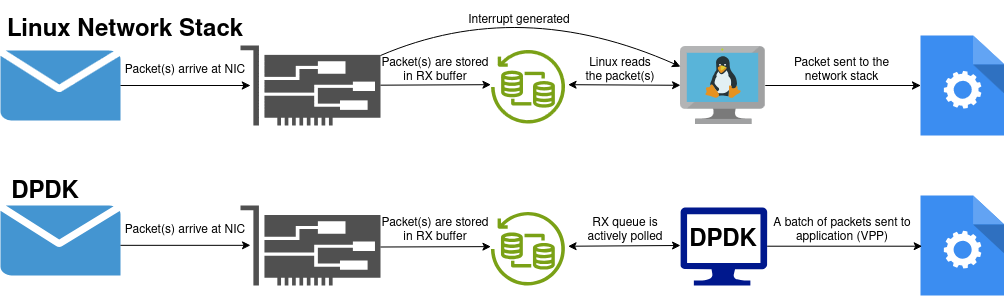
\includegraphics[width=0.99\linewidth]{images/dpdk-vs-linux.png}
    \caption{Diagram illustrating the differences in packet handling between the Linux Network Stack and DPDK}
    \label{fig:dpdk}
\end{figure}

%COMPARISON
Based on the description above, several key differences between the Linux Network Stack and DPDK can be observed.
Although both rely on a similar underlying mechanism -- ring buffer queues -- their implementations differ fundamentally.
In the Linux Network Stack, memory management is handled by the kernel through device drivers. 
In contrast, DPDK allocates memory in user space and manages it through its own framework, providing packet buffers and ring structures directly to the application.

Linux is heavily dependent on hardware interrupts (IRQs) for packet reception and software interrupts (softIRQs) for deferred processing, which introduces frequent context switches. 
While NAPI uses polling to process packets from receive queues, the packets are still handled by kernel strictly one by one.
This increases the likelihood of cache misses during packet processing, as each packet is processed independently and may not benefit from cache locality.

In contrast, DPDK works entirely in user space and uses continuous active polling, completely bypassing the need for interrupts and context switching. 
Since it does not wait for an interrupt to occur, packet processing can begin sooner, reducing initial latency. 
Additionally, DPDK can retrieve multiple packets in a single burst, preparing them for vectorized processing in VPP.
Figure \ref{fig:dpdk} presents a simplified diagram highlighting the key differences.


